%!TEX root = thesis.tex

\chapter{Background}
\label{part:literature}
    This chapter provides a discussion of the background and motivation of this work in further depth than the manuscripts in this dissertation.  Here, a general overview of ignitions as a threat to structures and fire spread as well as the current state of knowledge and predictive capabilities is communicated. Each manuscript includes a relevant and more detailed literature review pertaining to the specific objective of the work. 

    Wild fires have been an integral part of many ecosystems for millennia and are often beneficial or required for maintaining a healthy ecosystem. As beneficial as they may be to the natural enviornment wildfires pose significant risk to the built environment. As communities around the world have expanded communities outward into environments that support wildfires (e.g., forests and grasslands) the risk of destruction of structures by wildfires has increased. In the United States 91\% of the Wildland Urban Interface \nomenclature{WUI}{Wildland Urban Interface} growth of 189,000\si{\kilo\meter\squared} (larger than the state of Washington) development between 1990 and 2010 is occupied by homes~\cite{Radeloff2017} and has continued to grow on recent years. The increased development in theses areas means that an excess of 40 million homes are located in areas that may be threatened by a wildfire. 
    
    In addition to the increase of homes in the WUI the intensity and severity of fires has increased. California is a prime example of the increased fire severity where 13 of the 20 most destructive fires have occurred since 2010 and 7 of the 20 most destructive occurred in 2020 and 2021~\cite{CALFIRE2018}. Increasingly severe fires are not just limited to California or the United States. Texas and Tennessee each had one of the top ten most severe fires in the United States between 2005 and 2020 and Colorado, Oregon, Washington, Oklahoma, and Florida have also seen highly destructive fires in recent years~\cite{Barrett2020}. The United States is not unique in the presence of wilfdires that destroy homes. Australia's Black Summer in 2019-2020 was one of the most severe in the countries history~\cite{Levin2021}. The Mediterranean countries of Portugal, Spain, France, Italy, and Greece are also either experiencing greater losses or are a risk for greater losses due to wildfires in recent years. Similar trends are also present in many Asian and South American countries~\cite{Manzello2018}. Wildfires that threaten lives, homes, and structures are truly a global phenomena and it is essential to understand how homes are ignited and destroyed in wildfires to better prevent losses from occurring. 
    
    Ignition of a home in a WUI fire is attributed to three primary mechanisms; direct flame contact, ignition by radiative heating, and ignition by firebrands. Of these methods ignition by firebrands is considered to be a primary threat to homes~\cite{Suzuki2021, Mell2010}. A case study of structure ignitions in a WUI fire found that firebrand ignition was responsible for 2/3 of structure ignitions~\cite{Mell2011}. With the majority of ignitions occurring due to firebrand ignition it is imperative to understand the mechanism of firebrand ignition to reduce home losses. The general mechanism for firebrand ignition is considered to be a three step process which starts within the fire itself, often at a significant distance from the ignition point. First, a firebrand is generated as burning material breaks off or is lofted into the air. The firebrand is then lofted through the air and transported to the ignition site. Upon landing on a recipient fuel bed ignition occurs if the criteria for ignition is met~\cite{Babrauskas2003}. When considering the possibility of ignition during a fire event all three of processes must be considered as each process significantly influences the properties of an ember landing on a fuel bed. Due to the highly variable nature of winds that transport firebrands during fires the firebrand the firebrand generation and fuel bed ignition processes may be the most consistent when considering prevention approaches. Foliage types are much more consistent and measureable than wind and have a significant impact on the type of embers produced~\cite{Hudson2020EffectsScale} and fuel beds are largely controlled and/or modifiable by homeowners. Unfortunately, the generation and ignition processes are significantly less understood than the transport processes~\cite{Manzello2020}. The work contained in this dissertation is focused on the ignition process of the fuel bed by a firebrand and does not consider the generation of firebrands. For further information on firebrand generation processes the reader is referred to review papers considering this process by Fernandez-Pello~\cite{Fernandez-Pello2017} and by Manzello et al.~\cite{Manzello2020}.
    
    Developing and increased understanding of the ignition of a fuel bed has been identified as a necessary step to better protect structures from firebrand ignition for decades but research was limited until the mid 2000's. Early research and a significant portion of current research has been conducted by dropping combusting firebrands (either flaming or glowing) or hot metal particles fuel beds in varying configurations that simulate conditions in a wildfire and observing ignition or no ignition outcomes. These works have identified some parameters that appear to control ignition but models created from these studies only provide qualitative predictions of ignition. The lack of models of quantitative accuracy was suggested by Finney et al. in 2013 who identified the lack of a fundamental understanding of what processes occur and how they interact as a primary gap in the knowledge of ignition~\cite{Finney2013}. A similar need was identified by Manzello et al. in 2018~\cite{Manzello2018} and as recently as 2020~\cite{Manzello2020}. As the fires increase in severity and the number of homes is likely to keep increasing in the future the need for a better understanding of the processes the control ignition has never been more urgent.
    
    In order to identify the controlling parameters of ignition and create a model of quantitative accuracy the processes that occur leading up to ignition must be identified. Figure~\ref{fig:ignitionDiagram} illustrates the different factors that can influence the ignition process. To better understand how these parameters effect the ignition process can be considered as a series of three processes.  The first is the heat transfer to the fuel bed from the ember. The second is the pyrolysis of the fuel bed material and the subsequent release of pyrolyzates into the air above the fuel bed. The third step is the mixing of the pyrolyzates with air above the fuel bed and subsequent gas phase ignition. It is important to note that all three of these processes may occur simultaneously throughout the ignition process and are often interconnected. For example, as heat is transferred from the firebrand to the fuel bed the thermal conductivity of the fuel bed changes with temperature both before and after pyrolysis begins~\cite{Fjellerup2003}. Furthermore, the contact area between the firebrand and fuel continuously changes as mass is released due to pyrolysis. Due to the interconnection of the processes that occur during ignition and the inherent variability of fuel beds and biomass fuels in general quantification of parameters that influence ignition is quite challenging. Despite these challenges results of previous research have identified influential parameters that have consistently been observed to control ignition. This work considers these parameters as belonging to one of three categories namely, thermo-physical properties of the fuel bed, energy supplied by the firebrand, and environmental conditions near the ignition point. Detailed reviews of each category are provided in the relevant manuscripts and are not reproduced here. The remaining sections of this review address the predictive models of ignition that have been created from the current state of knowledge. The accuracy and appilicability of each model is discussed in turn and the remaining challenges are identified as they have motivated the objectives of this work. 
    
         \begin{figure}[hpbt]
            \centering
                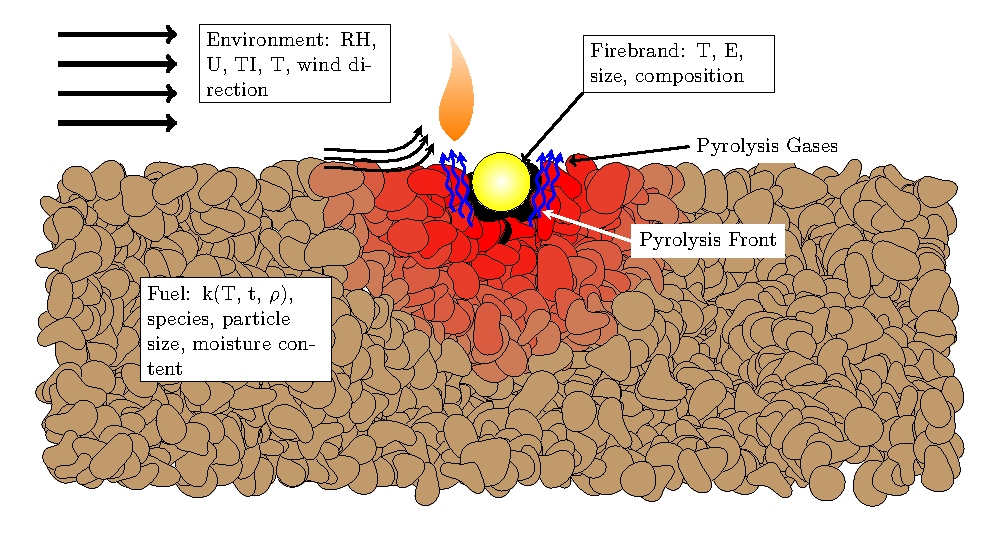
\includegraphics[width=0.75\textwidth]{Figures/dissertationBed.pdf}
            \caption{Diagram illustrating potential parameters that may influence ignition of a fuel bed.}
            \label{fig:ignitionDiagram}
        \end{figure}
    A significant number of ignition criteria and models have been proposed to predict fuel bed ignition, however no model has provided a general quantitatively accurate prediction of ignition. 
    \section{Current Ignition Models}
        \begin{itemize}
            \item Hot spot theory (Hadden 2011)
            \item Critical mass flux (Nelson 1995)
            \item Energy content of the particle
            \item Numerical methods
            \item Analytic correlations
        \end{itemize}
    
    %     \section{Energy Effects}
    %     Fuel bed response to heating and the impacts that heat transfer has on ignition probability is important knowledge for understanding ignition of fuel beds. Unfortunately, the current state of knowledge can only answer this question qualitatively. When looking at a fuel bed's response to incident heating, there are two major parameters that can be changed: the total amount of energy deposited to a fuel bed and the rate at which energy is deposited. Intuitively, increasing both of these parameters should increase the probability of ignition. Results from literature support this reasoning where increasing the energy deposition and/or the heat transfer rate increased the probability of ignition. Table~\ref{tab:binary} provides a summary of experimental efforts that have considered the ignition probability of fuel beds. For each study in Table~\ref{tab:binary} the fuel bed material, heat source, and parameters varied are outlined. The relative increase or decrease in ignition probability for each parameter change is also identified.
  

    %   \begin{table}[htbp]
    %          \rowcolors{2}{gray!25}{white}
    %          \caption{Summary of studies that have considered ignition probability of fuel beds. $\downarrow$ signifies an decrease in value and $\uparrow$ an increase}
    %             \centering
    %             \begin{tabular}{N p{1.5cm} p{3cm} p{3cm} p{4.5cm} p{0.7cm}}
    %             \rowcolor{gray!50}
    %                 \multicolumn{1}{|c}{ID} &  Fuel Bed & Heat Source & Parameter(s) & $\uparrow$ Ignition Probability & Ref  \\
    %                  \hline
    %                 \label{tabrow:wang2017}&             pine needles & metal  & FMC, $T_{ember}$, $U_{wind}$ \nomenclature{$U_{wind}$}{Air velocity over the fuel bed} & $\downarrow$ FMC, $\uparrow T_{ember}$ \nomenclature{$T_{ember}$}{Temperature of the ember}, $\uparrow U_{wind}$  & \cite{Wang2017}\\
                    
    %                 \label{tabrow:urban2017}&            powdered grass & metal &   $T_{ember}$, $d_{ember}$ \nomenclature{$d_{ember}$}{Ember diameter} & $\downarrow d_{ember}$ requires $\uparrow T_{ember}$ & \cite{Urban2017}\\
                    
    %                 \label{tabrow:Fernandez-Pello2015}&  cellulose & metal &     $T_{ember}$, $d_{ember}$ & $\downarrow d_{ember}$ requires $\uparrow T_{ember}$ & \cite{Fernandez-Pello2015}\\
                    
    %                 \label{tabrow:ellis2015}&            forest litter & glowing or flaming wood & flaming or glowing ember, FMC,  $U_{wind}$ &  $\uparrow U_{wind}$, $\downarrow$ FMC & \cite{Ellis2015}\\
                    
    %                 \label{tabrow:santoni2014}&          pine needles & radiative & $A_{s}/V$, permeability & $\uparrow A_{s}/V$ \nomenclature{$A_{s}$}{Surface area of the ember} \nomenclature{$V$}{Ember Volume}, $\uparrow$ permeability & \cite{Santoni2014}\\
                    
    %                 \label{tabrow:reszka2012}&           nylon, PMMA & radiative & heating rate & $\uparrow$ heating rate & \cite{Reszka2012}\\
                    
    %                 \label{tabrow:hadden2011}&           cellulose & metal & $T_{ember}$, $d_{ember}$ & $\downarrow d_{ember}$ requires $\uparrow T_{ember}$ & \cite{Hadden2011}\\
                    
    %                 \label{tabrow:ellis2011}&            forest litter & flaming bark & FMC, $U_{wind}$, glowing mass &  $\downarrow$ FMC, $\uparrow$ glowing mass, $\uparrow U_{wind}$ & \cite{Ellis2011}\\
                    
    %                 \label{tabrow:ganteaume2009}&        forest litter & flaming wood & $\rho$, FMC, species & $\downarrow$ FMC, $\downarrow \; \rho$ , species effect & \cite{Ganteaume2009}\\
                    
    %                 \label{tabrow:plucinski2008}&        forest litter & cotton balls, aerial incendiary & FMC, species, $U_{wind}$ &  $\downarrow$ FMC, species effect, wind effect,  $\uparrow E_{ember}$\nomenclature{$E_{ember}$}{Energy content of ember}& \cite{Plucinski2008}\\
                    
    %                 \label{tabrow:manzello2006}&         litter, paper, crevices & glowing/flaming wood & $U_{wind}$, FMC, $d_{ember}$, $N_{ember}$ \nomenclature{$N_{ember}$}{Number of embers} & material effect, flaming/glowing, $\downarrow$ FMC,  $\uparrow N_{ember}$ & \cite{Manzello2006}\\
                    
    %                 \label{tabrow:manzello2006a}&        various mulches & glowing/flaming wood &  $U_{wind}$, FMC, $d_{ember}$ & material effect, flaming/glowing, $\downarrow$ FMC, $\uparrow U_{wind}$,  $\uparrow N_{ember}$ & \cite{Manzello2006a}\\
                    
    %                 \label{tabrow:yang2003}&             wood plates & radiative & heat flux & $\uparrow$ heat flux & \cite{Yang2003}\\
                    
    %                 \label{tabrow:delichatsios}&         wood plates & radiative & heat flux & $\uparrow$ heat flux & \cite{Delichatsios2003}\\
                    
    %                 \label{tabrow:dimitrakopoulos2001a}&  various leaf species & radiative & FMC, species & species dependence, $\downarrow$ FMC & \cite{Dimitrakopoulos2001a}
    %             \end{tabular}
    %             \label{tab:binary}
    %             \end{table}


    %     Experiments conducted by Fernandez-Pello et al.~\cite{Fernandez-Pello2015}, in which hot metal particles were dropped onto cellulose, indicated the determining factor for ignition was proportional to the energy of the firebrand. More specifically, ignition was observed if the amount of thermal energy available from the particle delivered enough energy such that sufficient pyrolyzates were generated. This relationship manifests as a parabolic relationship between the particle diameter and energy of the particle at the ignition boundary as shown in Figure~\ref{fig:energy_diameter}. 
    %         \begin{figure}[hpbt]
    %             \centering
    %             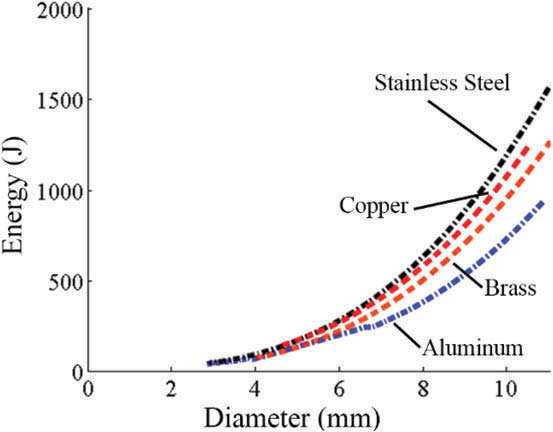
\includegraphics[width=0.5\textwidth]{Figures/particle_ign_boundary.png}
    %             \caption{Observed ignition boundary, quantified by particle energy, as a function for cellulose powder for various materials and particle sizes from Fernandez-Pello et al.~\cite{Fernandez-Pello2015}.}
    %             \label{fig:energy_diameter}
    %         \end{figure}
    %     Similar results for hot particles were obtained for pine needles by Wang et al.~\cite{Wang2017}, for powdered grass by Urban et al.~\cite{Urban2017}, and again with cellulose by Hadden et al.~\cite{Hadden2011}. While similar trends have been observed across a range of materials using similar energy delivery methods, efforts to create a model to predict ignition boundaries have not been successful. The difficulties preventing an ignition model have stemmed from the lack of knowledge about the ember fuel bed interface, thermal properties of the fuel bed, and difficulties in determining particle heat losses to ambient. 
        
    %     While observations informing trends that increased energy and heat transfer increase  probability are important, the next step is to quantify the transition or critical values for parameters observed to control the trends. A universally predictable critical value has not yet been determined but, predictive capabilities for single conditions or experimental apparatus have been determined. More detail on what has been learned about the impact of energy deposition and effects of energy deposition on pyrolysis is contained in the following sections.
        
    %     \section{Fuel Moisture Content}
    %     The presence of water in fuel bed particles, quantified as fuel moisture content, impacts the ignition process in multiple ways. Since the vaporization of water occurs at a lower temperature than pyrolysis, the water in a fuel particle must be evaporated before pyrolysis can occur. This creates a large energy sink for the energy imparted to the fuel bed from an ember or firebrand, thus increasing the amount of energy needed to ignite a fuel bed~\cite{Hurley2016}. Studies have universally shown this to be the case as is described in Table~\ref{tab:binary} rows~\ref{tabrow:wang2017}, \ref{tabrow:ellis2015}, \ref{tabrow:ellis2011}, \ref{tabrow:ganteaume2009}, \ref{tabrow:plucinski2008}, \ref{tabrow:manzello2006}, \ref{tabrow:manzello2006a}, and~\ref{tabrow:dimitrakopoulos2001}. This trend indicates that fuel moisture content is a parameter to be added as a lumped constant to the minimum energy needed to ignite a fuel bed. However, water in the fuel has additional impacts on the pyrolysis and ignition processes. Computational efforts have shown that increasing the moisture content of the fuel decreases both the peak mass loss rate and peak heat release rate of a fuel sample\cite{Shotorban2018}. The decrease in the heat release rate and mass loss rate may have significant effects on the chemical composition of the pyrolysis gases, as was observed by Furgeson et al.~\cite{Ferguson2013} where an increased moisture content shifted the \ce{O2} and \ce{H} concentrations in flames burning pyrolysis gases. It should be noted that this effect was observed for the piloted combustion of pyrolysis gases, but increasing amounts of \ce{H2O} would likely have a similar impact on the auto-ignition of pyrolysis gases. The implications of these effects are discussed further in Section~\ref{subsec:pyrolysis}, as they relate more directly to pyrolysis of the fuel and gas dynamics above the fuel bed. 
        
    %     In addition to acting as an energy sink for evaporation, increasing the fuel moisture content alters the thermal conductivity of a fuel bed. Tests for the thermal conductivity of wheat showed that a 28\% increase in wheat moisture content increased the thermal conductivity by ~40\%\cite{Tavman1998}. The increased heat diffusion rates would lead to lower temperatures and temperature gradients in the fuel bed, changing the mass flux rate of pyrolyzates departing the fuel bed and the composition of said pyrolyzates. The relative magnitude of increased moisture content in other fuel bed materials is unclear, but a ~40\% shift in thermal conductivity would have significant impacts on the heat diffusion rates from a firebrand delivering energy to the fuel bed.
    %     Perhaps the most important knowledge gained from the extensive study of fuel moisture content and its impacts is that due to the numerous scales across which ignition of fuel beds occur it is essential to evaluate the impacts of each parameter across all scales since the phenomena may be more closely interdependent than initially observed. 
            
    %     \section{Species and Morphology}
    %     One of the factors that sets the ignition of fuel beds apart from ignition of other materials is the vast array of species and particle morphology encountered in nature. For example, in a forest with a relatively uniform litter layer, the particle size distribution may range from small pieces of grass to twigs that are an order of magnitude larger. Even a layer of pine needles on a roof will have a distribution of sizes, shape, orientation, and bulk density. On the scale of the fuel bed, the differences in shapes and sizes of the particles ensure that every fuel bed is unique, making repeatability while studying fuel bed ignition difficult at best. 
        
    %     Implications for fuel bed uniqueness is twofold. First, the differences in particle shape, e.g., pine needles vs oak leaves, cause the heat transfer properties of fuel beds to be highly variable. Second, each species has different composition and fuel beds may consist of many species. Having fuel bed particles of different compositions and morphology in a fuel bed obfuscates the relative effects of individual particle thermal conductivity and inter-particle heat transfer due to contact area and particle shape. Furthermore, a fuel bed with multiple species will undergo a wide array of chemical processes in a single fuel bed when pyrolyzates are generated. Samples of the same fuel have also been shown to have different pyrolyzate composition under differing heating conditions~\cite{Gauthier2013}. For example, decreasing the heating source from 1050$^{\circ}$C to 450$^{\circ}$C reduced the elemental composition of hydrogen in the pyrolysis products by 23\% and increased the elemental composition of oxygen by 28\% on a \% mole basis. The inherent variability in natural fuel bed has limited observations to qualitative trends.
        
        
    %     Fortunately, despite the large variability across species and materials, there are three major components that are common across most biomass fuels: cellulose, hemicellulose, and lignin. Recent efforts, supported by the large amount of data produced by the previously mentioned studies, have attempted to find a common characterization for biomass materials by comparing composition differences. It was found that characterization of cellulose, hemicellulose, and lignin composition was not sufficient and extractive compounds must be considered. When extractive compounds were considered, chemical kinetic properties were able to be predicted within accuracy of existing models~\cite{Debiagi2015} with more detailed characterizations. This development helps lessen some of the difficulties encountered in previous studies by enabling the comparison of different species with less intensive methods of characterization. The ability for this approach to increase comparability between tests is a significant step forward in the understanding of ignition. However, there remains a multitude of effects on ignition introduced by species and morphology that need to be considered. These effects are outlined and considered in the following section. 
        
    %     \section{Pyrolysis Production and Air Mixing}\label{subsec:pyrolysis}
    %     Pyrolysis of fuel bed material is the keystone process for the ignition of fuel beds. Once the heat transfer to the fuel bed raises the temperature of the fuel enough for pyrolysis to occur, a number of conditions must be met for the ignition to occur.  The thermal degradation reactions that occur at the onset of pyrolysis are heavily influenced by the parameters discussed in the previous sections. The rate of energy deposition, fuel moisture content, species, and fuel morphology all modify the rate and composition of pyrolysis products. 
    %     The heating rate and the overall energy imparted to the fuel bed have the most prominent effect on the pyrolysis reactions in a fuel bed. At low temperatures and low heating rates the main components released by the fuel bed consist of chars, tars, and other large hydrocarbon chain molecules due to incomplete breakdown of the materials. As temperatures increase the products shift to more complete reactions that increase the amount of \ce{CO}, \ce{CO2}, \ce{H2}, and small hydrocarbons produced~\cite{Gauthier2013}. An example of this effect is shown in Figure~\ref{fig:temp_effects_pyrolysis} where small wood particles were placed in a heating apparatus at various temperatures. 
    %         \begin{figure}
    %             \centering
    %             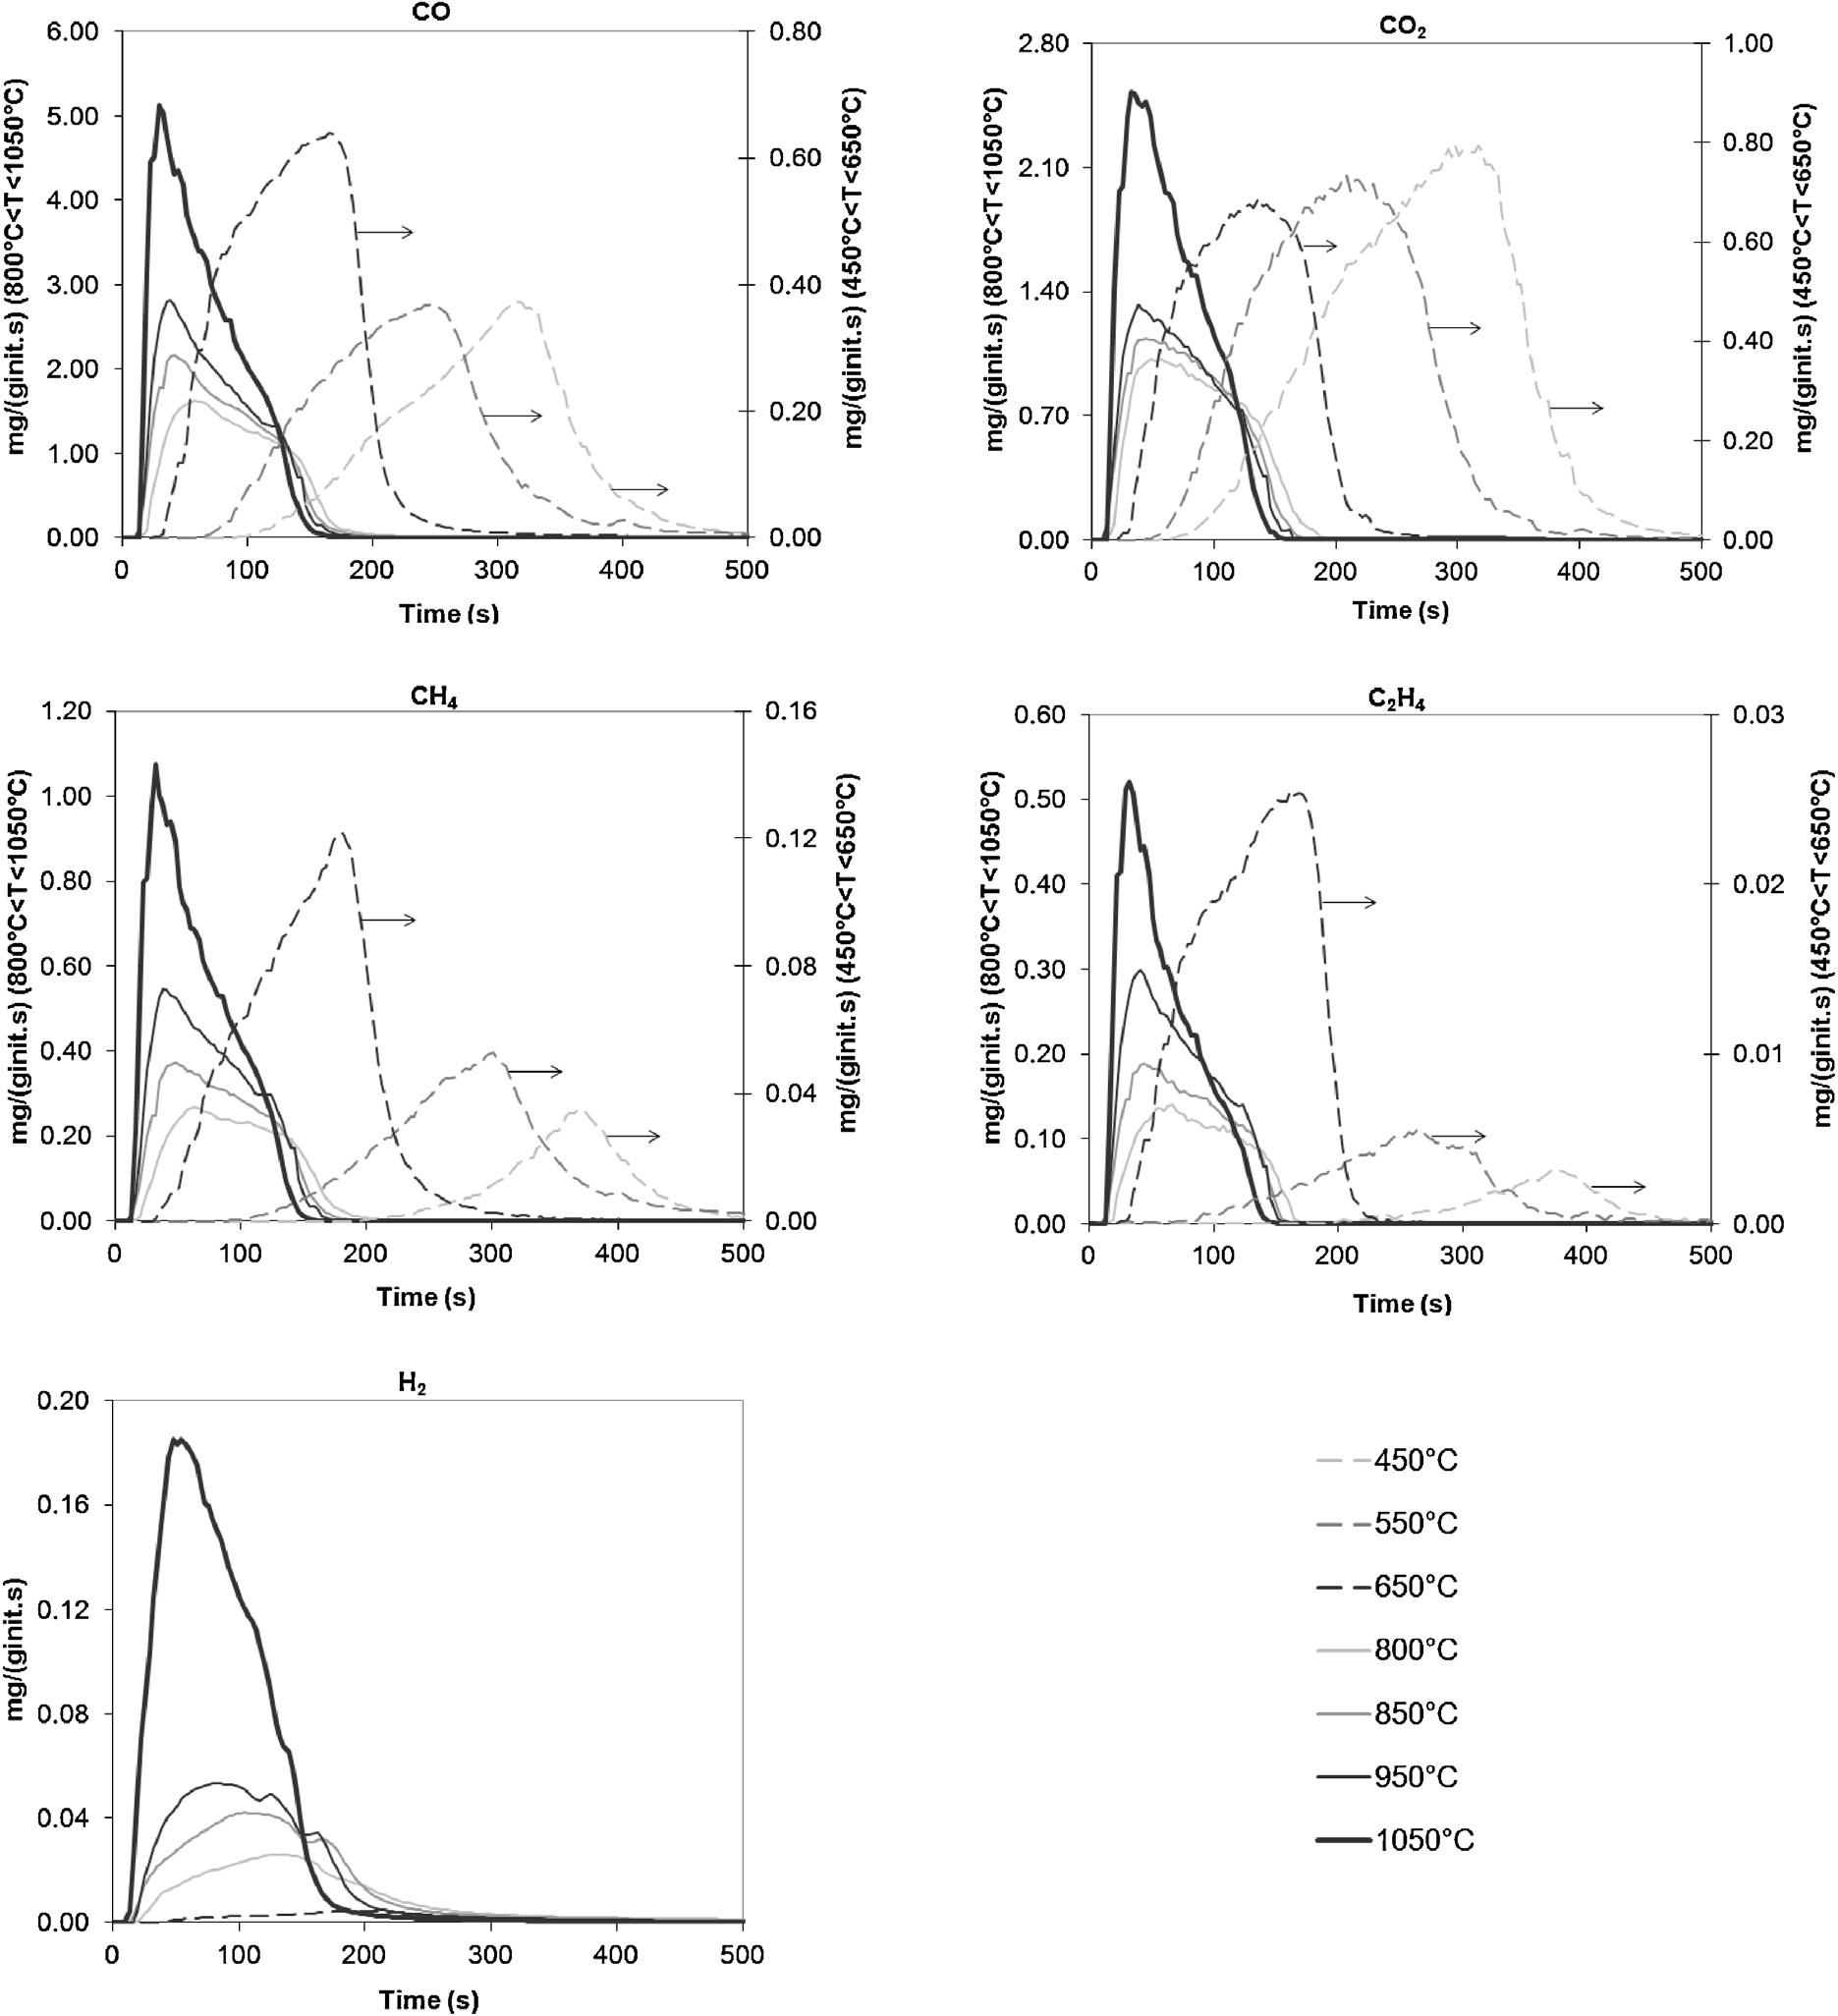
\includegraphics[width=0.75\textwidth]{Figures/gauthier2013_temp_effects.png}
    %             \caption{Pyrolysis gas concentrations for beech wood samples heated at different rates from ~\cite{Gauthier2013} showing the significant decrease in gas production rates for most gases as the sample temperature decreases.}
    %             \label{fig:temp_effects_pyrolysis}
    %         \end{figure}
    %     As is shown in Figure~\ref{fig:temp_effects_pyrolysis}, the heating rate affects both the rate of gas productions and the total amount of gas production. These trends have significant implications for ignition of pyrolysis gases above the fuel bed, since auto-ignition is dependent on the temperature, concentration, and species of the gases in the above the fuel bed.
        
    %     Similar trends have been observed for larger solid plates of plastics and wood in a wind tunnel with piloted flame. It was observed that under higher heat fluxes, the ignition time was shorter but the amount of pyrolyzates generated per time increases. The rate of pyrolyzate generation above which ignition was observed is considered to be the critical mass flux. This phenomena has been observed consistently across plastic and wood plates, as well as pine needles~\cite{McAllister2013, Hernandez2018}. The increase in the critical mass flux for ignition is attributed to higher temperature gradients in the material, causing most of the chemical reactions to occur near the surface of the material at a higher oxygen content and temperature~\cite{Rich2007}. Reactions under these condition produce more \ce{CO} and \ce{CO2}, as shown in Figure~\ref{fig:temp_effects_pyrolysis}, which have a increased lower flammability limit than larger hydrocarbons produced at lower heat fluxes. What is not clear from these findings is how fuel beds of different materials compare to solid fuels under the same conditions or the effects of different heat transfer modes. As particle sizes increase, the properties of the fuel bed become further from a solid as the porosity, surface area, and oxygen availability increase. The converse of these increases is a likely drop in bulk fuel bed thermal conductivity, creating higher temperature gradients. These temperature gradients have been shown to have change pyrolyzate composition for very small sample sizes ($\leq$10mg) in highly controlled Thermogravametric Analysis (TGA) tests~\cite{Richter2018}. While it is apparent that temperature gradients in the fuel bed affect pyrolyzate production, it is unclear how this will effect ignition of the fuel bed on scales found in fires. For these larger fuel beds, distributions of temperature and species concentrations caused by non-uniform and multiple heat sources is an important factor to understand when considering ignition. 
        
    %     Entrainment and mixing of air with pyrolyzates above the fuel bed has a pronounced effect on the ignition of fuel beds. As shown in Table~\ref{tab:binary} rows~\ref{tabrow:wang2017}, \ref{tabrow:ellis2015}, \ref{tabrow:ellis2011}, \ref{tabrow:plucinski2008} studies of fuel bed ignition that considered variable wind speed reported that an increase in wind speed increased the probability of ignition with other factors held constant. Increasing the flow velocity above the fuel bed reduces both the relative importance of buoyant forces and the timescale for mixing. With increased velocity and turbulence, air and pyrolyzates mix faster but heat loss to increased air advection also increases. The relative magnitude of time scales between heat and species diffusion in reacting flows are commonly compared using the Damkohler number as shown in Equation~\ref{eqn:dam}.
        
    %         \begin{equation}\label{eqn:dam}
    %             \text{Da} = \frac{\text{flow time scale}}{\text{chemical time scale}}
    %         \end{equation}
    %     In the Damkohler number, the flow velocity and turbulence that affect the mixing of air and pyrolyzates are considered in the flow time scale term.  The chemical time scale term considers the pyrolyzate species concentration and temperature effects. The interaction of these two terms is well defined and commonly used in combustion to determine flame regimes and ignition. Use of the Damkohler number as a relation to define ignition has seen limited use in ignition of fuel beds since the knowledge of species concentrations, temperatures, and air flow effects are largely unknown. Gaining insight into these effects would enable the use of tools like the Damkohler number to successfully predict ignition across a variety of fuel beds. 
    %     Namely, quantification of the parameters near the fuel bed (e.g., surface wind speed), fuel properties (e.g., chemical composition, estimated ember contact area), and the energy content of a firebrand may enable a common metric to predict if ignition will occur in a fire without ignition testing for a certain specific fuel, set of conditions, and location.
    %     \section{Summary}
    %     Substantial progress has been made to further the understanding of fuel bed ignition and the effects of various related parameters. Despite these efforts, there remains no universal or even quantitative approach that can be used to effectively predict ignition of fuel beds without prior testing for a specific source or fuel. Current knowledge is capable of predicting ignition of solids and predicting different pyrolysis properties of fuels, but the knowledge has not been extended to fuel beds that may occur in forest fires and near structures. One of the largest gaps in knowledge that remains is to determine how fuel beds that consist of fine fuel particles behave in comparison to solid theory. In addition, the effects of non-uniform heating and variable energy deposition are largely unknown. In order to close these knowledge gaps three avenues of research are proposed. First, the heat transfer properties of the fuel bed must be quantified to obtain better knowledge of how the fuel bed responds to heating. Second, the generation rates of pyrolyzates and the effect that heating rates, heat source temperatures, and heating modes must be quantified. Third, the mixing timescales between the pyrolyzates and air must be evaluated to determine what rate the pyrolyzates must be generated to achieve ignition across a variety of conditions. This approach will help bridge the gap between the fundamental theories for ignition and real fuel beds where wildfires occur. The approach and methodologies for each of these fundamental processes is outlined in the following sections. 
        
        
  
